%%
%%  Hochschule für Technik und Wirtschaft Berlin --  Abschlussarbeit
%%
%%  Hauptdokument
%%
%%%%%%%%%%%%%%%%%%%%%%%%%%%%%%%%%%%%%%%%%%%%%%%%%%%

%% Einstellungen und Anpassungen
% Wichtige Pakete und Grundeinstellungen, verwendet Dokumentenklasse "scrbook" 
\documentclass[
		chapterprefix=false, 
		a4paper, 
		twoside, 
		parskip=half, 
		listof=totoc, 
		bibliography=totoc, 
		numbers=noendperiod, 
		captions=tableheading
]{scrbook}

%Anpassung der Seitenränder 
%% Geometrisches ...
\usepackage[inner=3cm]{geometry}
\makeatletter
\setlength\paperheight     {297mm}
\setlength\paperwidth  	   {210mm}
%\setlength\headheight      {2ex}
\setlength\headsep         {4ex} %2
\setlength\footskip        {35pt} %25
\setlength\textwidth       {155mm}
\setlength\textheight      {240mm} %245
%\setlength{\@tempdima}     {\paperwidth}
%\addtolength{\@tempdima}   {-2in}
%\addtolength{\@tempdima}   {-\textwidth}
%\setlength\oddsidemargin   {0.5\@tempdima} %replaced by 'inner'
%\setlength\evensidemargin  {\oddsidemargin} %replaced by 'inner'
%\setlength{\@tempdima}     {\paperheight}
%\addtolength{\@tempdima}   {-3in}
%\addtolength{\@tempdima}   {-\textheight}
%\setlength\topmargin       {.5\@tempdima}
\setlength\topmargin       {-1,2cm}
\setlength\footnotesep     {12\p@}
\setlength{\skip\footins}  {10\p@ \@plus 2\p@ \@minus 4\p@}
\setlength{\marginparsep}  {1pt}
\setlength{\marginparwidth}{20mm}
\makeatother 


%% Scalable fonts
\usepackage{lmodern}
%% set font size (needs to be loaded after \begin{document})
\AtBeginDocument{%
  \KOMAoption{fontsize}{11.5pt}%
%  \recalctypearea % not needed because use of geometry package
}
%% Unterstützung von Umlauten und anderen Sonderzeichen (UTF-8)
\usepackage{eurosym}
\usepackage[utf8]{inputenc}
\usepackage[T1]{fontenc}
\DeclareUnicodeCharacter{20AC}{\euro} %Euro-Symbol in UTF-8

%% Allgemeine Anpassungen 
\usepackage{scrhack} %Tweaks für scrbook
\usepackage[automark,headsepline]{scrlayer-scrpage} %Anpassung von Kopf- und Fußzeile
\usepackage{paralist}  %Kompakte Listen
%\usepackage[onehalfspacing]{setspace} %Zeilenabstand 1,5
\usepackage{setspace} %flexibler Zeilenabstand
\setstretch{1.15} %Zeilenabstand 1.1

\usepackage[stretch=10]{microtype} %Verbesserte Darstellung der Buchstaben zueinander
\usepackage{float} %Unterstützung fester Positionierung  (H)
\usepackage{csquotes} %wird von babel benötigt

%Glossar, Stichworverzeichnis (Akronyme als eigene Liste)
%\usepackage[toc, acronym]{glossaries} 

%% Mathematik:
\RequirePackage{amssymb, amsmath}
\RequirePackage{ifthen}
\RequirePackage{pifont} % Zapf Dingbats : https://ctan.ebinger.cc/tex-archive/macros/latex/required/psnfss/psnfss2e.pdf

%% Erweiterte Tabellen:
\usepackage{array, tabularx}
\setlength\extrarowheight{2pt} %extra Top-Padding in Latex-Tabellen
\usepackage{multirow}
\usepackage{longtable} %Umbrüche in Tabellen

%% Grafiken:
% Definition eigener Farben 
\usepackage[table,xcdraw]{xcolor}
\usepackage{tikz} % Vektorgrafiken, lädt graphicx automatisch
\usepackage{bmpsize} 

%Verknüpfungen im Dokument, Links werden durch "hidelink" nicht explizit hervorgehoben
%\PassOptionsToPackage{hyphens}{url}
\usepackage[hidelinks,german,hypertexnames=false]{hyperref}
%\hypersetup{breaklinks=true}
\usepackage{breakurl}
%\expandafter\def\expandafter\UrlBreaks\expandafter{\UrlBreaks% save the current one
%  \do\a\do\b\do\c\do\d\do\e\do\f\do\g\do\h\do\i\do\j%
%  \do\k\do\l\do\m\do\n\do\o\do\p\do\q\do\r\do\s\do\t%
%  \do\u\do\v\do\w\do\x\do\y\do\z\do\A\do\B\do\C\do\D%
%  \do\E\do\F\do\G\do\H\do\I\do\J\do\K\do\L\do\M\do\N%
%  \do\O\do\P\do\Q\do\R\do\S\do\T\do\U\do\V\do\W\do\X%
%  \do\Y\do\Z\do\*\do\-\do\~\do\'\do\"\do\-}%
  		% Import der Pakete und Stil des Dokuments
%%% Einstellungen zur Sprache und Silbentrennung im Dokument
%
% This is a document holding multiple languages.
% Switch between ENGLISH and GERMAN by commenting one of the following lines:
%\usepackage[ngerman,english]{babel} % makes ENGLISH content
\usepackage[english,ngerman]{babel} % makes GERMAN content
% this is the macro to define phrases in two languages:
\newcommand{\babel}[2]{\ifnum\pdfstrcmp{\languagename}{english}=0 {#2}\else{#1}\fi}
\newcommand{\DE}[1]{\ifnum\pdfstrcmp{\languagename}{ngerman}=0 {#1}\fi}
\newcommand{\EN}[1]{\ifnum\pdfstrcmp{\languagename}{english}=0 {#1}\fi}
% example:   \babel{Deutscher Text}{english text}
% example:   \DE{deutscher Text}
% example:   \EN{english text}
%%%%%%%%%%%%%%%


%%% Erstellung von Literaturverzeichnissen mit Biblatex (Biber/Bibtex)
% wählen Sie hier die für Ihr Latex-System nötige Literaturverarbeitung:
\usepackage[style=alphabetic, backend=biber,   natbib=true]{biblatex}  % Verarbeitung mit biber
%\usepackage[style=alphabetic, backend=bibtex, natbib=true]{biblatex}  % Verarbeitung mit bibtex
%
% Bibtex-Datei mit den Quellenangaben zur Arbeit
\addbibresource{references/references.bib}


%%% Abkürzungsverzeichnis
\usepackage[intoc]{nomencl}
\let\acro\nomenclature
\renewcommand{\nomname}{\babel{Abkürzungsverzeichnis}{Abbreviations}}
\setlength{\nomlabelwidth}{.25\hsize}
\renewcommand{\nomlabel}[1]{#1 \dotfill}
\setlength{\nomitemsep}{-\parsep}
\makenomenclature

%%% Überschriften auch in Times-Roman setzen
\addtokomafont{disposition}{\rmfamily}

%%% Kapitelnummer und Titel auf einer Zeile (erfordert die chapterprefix=false Option in class)
\renewcommand*{\chapterformat}{%
  \mbox{\chapapp~\thechapter:\enskip}%
}

%%% Farbdefinitionen
%  https://corporatedesign.htw-berlin.de/schrift-farbe/markenfarben/
\definecolor{HKS66}{RGB}{118,185,0}          %% HKS51, HTW-Grün
\definecolor{HKS47}{RGB}{0,130,209}      %% HKS47, HTW-Blau
\newcommand{\headcolor}{HKS66}
\newcommand{\alertcolor}{HKS47}
% Zusätzliche Farben
\definecolor{darkgreen}{RGB}{0,100,0}


%%% Stichwortverzeichnis 
\usepackage{imakeidx}
\makeatletter
\makeindex[columns=2, title=\babel{Stichwortverzeichnis}{Index}, options= -s settings/indexstyle.ist, intoc]
\makeatother
\indexsetup{level=\chapter*,toclevel=chapter}
% Pluszeichen in der Referenz beim Zitieren entfernen: [Kra+13] wird zu [Kra13]
\renewcommand*{\labelalphaothers}{}


%%% Darstellung von Quellcode incl. Syntax-Highlighting
\usepackage{listings}
\renewcommand{\lstlistlistingname}{\babel{Quelltextverzeichnis}{Listings}}
%Anpassungen zur Quellcodedarstellung
% muss bei Bedarf überschrieben werden (z.B. wenn unterschiedliche Sprachen zum Einsatz kommen)
\renewcommand{\lstlistingname}{Codeauszug}
\lstset{
	language=Java,
	numbers=left,
	columns=fullflexible,
	aboveskip=5pt,
	belowskip=10pt,
	basicstyle=\small\ttfamily,
	backgroundcolor=\color{black!5},
	commentstyle=\color{darkgreen},
	keywordstyle=\color{blue},
	stringstyle=\color{gray},
	showspaces=false,
	showstringspaces=false,
	showtabs=false,
	xleftmargin=16pt,
	xrightmargin=0pt,
	framesep=5pt,
	framerule=3pt,
	frame=leftline,
	rulecolor=\color{green},
	tabsize=2,
	breaklines=true,
	breakatwhitespace=true,
	prebreak={\mbox{$\hookleftarrow$}}
}

 	% Weitere Pakete und Anpassungen (Sprache, Quellenverwaltung, etc.)

% Variablendefinition und deren Voreinstellung festlegen
%

%% Variablen
\newboolean{@entwurfset}        \setboolean{@entwurfset}{true}
\newboolean{@abgabeset}         \setboolean{@abgabeset}{true}
\newboolean{@versionset}        \setboolean{@versionset}{true}
\newboolean{@versionsdatum}      \setboolean{@versionsdatum}{true}

%
\newcommand{\version}[1]{\setboolean{@versionset}{true} 
 \renewcommand{\theversion}{#1}} 
\newcommand{\datum}[1]{\renewcommand{\thedatum}{#1}}
\newcommand{\autor}[1]{\renewcommand{\theautor}{#1}}
\newcommand{\matrikelnr}[1]{\renewcommand{\thematrikelnr}{#1}}
\newcommand{\titel}[1]{\renewcommand{\thetitel}{#1}}
\newcommand{\untertitel}[1]{\renewcommand{\theuntertitel}{#1}}
\newcommand{\fachbereich}[1]{\renewcommand{\thefachbereich}{#1}}
\newcommand{\studiengang}[1]{\renewcommand{\thestudiengang}{#1}}
\newcommand{\thesistyp}[1]{\renewcommand{\thethesistyp}{#1}}
\newcommand{\abschluss}[1]{\renewcommand{\theabschluss}{#1}}
\newcommand{\firstExaminer}[1]{\renewcommand{\thefirstExaminer}{#1}}
\newcommand{\secondExaminer}[1]{\renewcommand{\thesecondExaminer}{#1}}
\newcommand{\betreuerFeld}[1]{\renewcommand{\thebetreuerFeld}{#1}}

%
\newcommand{\theversion}{0.0}      
\newcommand{\thedatum}{\today}
\newcommand{\theautor}{Autor angeben!}
\newcommand{\thematrikelnr}{123 456}
\newcommand{\thetitel}{Titel angeben!}
\newcommand{\theuntertitel}{}
\newcommand{\thefachbereich}{Fachbereich angeben}
\newcommand{\thestudiengang}{Studiengang angeben}
\newcommand{\thethesistyp}{Bachelorarbeit}
\newcommand{\theabschluss}{Bachelor of Engineering (B.Eng.)}
\newcommand{\thefirstExaminer}{Betreuer 1}
\newcommand{\thesecondExaminer}{Betreuer 2}
\newcommand{\thebetreuerFeld}{}

\betreuerFeld{
  \begin{tabular}{llr}
    Erstgutachten: & \thefirstExaminer \\
    Zweitgutachten: & \thesecondExaminer \\
  \end{tabular}
}


%%%%%%%%%%%%%%%%%%%%%%%%%%%%%%%%
\renewcommand{\maketitle}{\htwTitelSeite}

%% Optionen

\DeclareOption{entwurf}
    {
      \setboolean{@entwurfset}{true}
      \setboolean{@abgabeset}{false}
    }

\DeclareOption{abgabe}
    {
      \setboolean{@entwurfset}{false}
      \setboolean{@abgabeset}{true}
    }



%% Setzen des defaults und verarbeiten
\ExecuteOptions{abgabe}     %TODO für Abgabe auf abgabe setzen
\ProcessOptions 

%%%%%%%%%%%%%%%%%%%%%%%%%%%%%%%%
%\newcommand{\hslogo}{pictures/Logo_HTW_Berlin.pdf}
%\newcommand{\hslogoscaled}[1]{{\mbox{\includegraphics[width=#1]\hslogo}}}

\newcommand{\hsfont}{}%    {\fontfamily{phv}\fontseries{m}\fontshape{n}\selectfont}
\newcommand{\hsheadfont}{}%{\fontfamily{phv}\fontseries{b}\fontshape{n}\selectfont}

\newcommand{\htwTitelSeite}
    {
      \thispagestyle{empty}
      \parindent=0pt
      \begin{minipage}[b]{0.65\textwidth}
       
        \ifthenelse{\boolean{@entwurfset}}
            {
              \begin{hsfont}
                \begin{tiny}
                  \raggedright
                  % Versionsnummer, wenn gesetzt
                  \ifthenelse{\boolean{@versionset}}
                       {Version \theversion\\}
                       {}
                       % Datum der letzten Änderung, falls gewünscht
	               \ifthenelse{\boolean{@versionsdatum}}
                       {letzte Änderung: \today \\}
		       {}
                \end{tiny}
              \end{hsfont}
            }
            {              
              % leer
              ~\hfill~
            }
      \end{minipage}
      
      \begin{minipage}[b]{0.35\textwidth}
      \vskip -2em
      \hfill  %\hslogoscaled{\textwidth}
%      \Ifpdfoutput{
%                  \message{PDF Output}
                  \mbox{
\includegraphics[width=\textwidth]{pictures/Logo_HTW_Berlin}}
%                  }{
%                 \mbox{
\includegraphics[width=\textwidth]{pictures/Logo_HTW_Berlin.eps}}
%                  \message{Kein PDF Output}
%                  }
      \end{minipage}

      \textcolor{HKS66}{\rule{\linewidth}{.4mm}}
      \vspace*{\stretch{1}}
      \begin{center}
        \begin{hsheadfont}
          \textcolor{\headcolor}{\LARGE \textbf{\thetitel}}
        \end{hsheadfont}
      \end{center}
      \vspace*{\stretch{0.5}}
      %
      \begin{hsheadfont}
        \begin{center}
          \textbf{\Large{\thethesistyp}}
        \end{center}
      \end{hsheadfont}
      \vspace*{\stretch{0.5}}
      %
      \begin{center}
        \begin{hsfont}
          von\\[2ex]
          {\textbf{\large\theautor}}\\[2ex]
          Matrikelnummer: \thematrikelnr\\[2ex]
          Fachbereich \thefachbereich\\
          der Hochschule für Technik und Wirtschaft Berlin\\[2ex]
          zur Erlangung des akademischen Grades\\
          \textbf{\theabschluss}\\
          im Studiengang\\
          \textbf{\thestudiengang}
        \end{hsfont}
      \end{center}
     
      \vspace*{\stretch{1}}
       \begin{center}
         Tag der Abgabe: \thedatum 
       \end{center}
         
      \vspace*{\stretch{1}}
      
      \thebetreuerFeld
      
      %
      \vspace*{\stretch{2}}

      \textcolor{HKS66}{\rule{\linewidth}{0.4mm}}\\[1.5ex]
       \begin{hsheadfont}
         % leer
         ~\hfill~
       \end{hsheadfont}
    }
    
		% Layout der Titelseite

%%%%%%%%%%%%%%%%%%%%%%%%%%%%%%%%%%%%%%%%%%%%%
%%%%%%%%%%%%%%%%%%%%%%%%%%%%%%%%%%%%%%%%%%%%%
%% Im folgenden Bereich müssen Sie Anpassungen für das Deckblatt der Arbeit vornehmen!
%
%% Titel und Author 
\titel{Analyse, Planung und Implementierung einer internetfähigen Steuerung}
\autor{Hans Maier}
\matrikelnr{s1234567}
%% Version und Abgabedatum
\version{0.2$\alpha$} 	%ToDo: wird derzeit noch nicht genutzt
\datum{07.04.2022}   	% Abgabedatum der Arbeit
%% Typ der Arbeit
\thesistyp{Masterarbeit}
%\thesistyp{Bachelorarbeit}
\abschluss{Master of Engineering (M. Eng.)}
%\abschluss{Bachelor of Engineering (B. Eng.)}
%% Betreuer
\firstExaminer{Prof.~Dr. Thomas Scheffler}
\secondExaminer{Maxi Mustermann}
%% Fachbereich
\fachbereich{1 -- Energie und Information --}
\studiengang{Informations- und Kommunikationstechnik}
%%%%%%%%%%%%%%%%%%%%%%%%%%%%%%%%%%%%%%%%%%%%%
%%%%%%%%%%%%%%%%%%%%%%%%%%%%%%%%%%%%%%%%%%%%%
%%%%%%%%%%%%%%%%%%%%%%%%%%%%%%%%%%%%%%%%%%%%%
%% Metadaten zu PDF hinzufügen
\hypersetup{
pdftitle = {\thetitel},
pdfsubject = {\thethesistyp},
pdfauthor = {\theautor},
%pdfkeywords = {Stichwort1, Stichwort2 ...} ,
pdfcreator = {LaTeX with hyperref},
pdfproducer = {pdflatex}
}
%% Pfad zu den Bildern
\graphicspath{
  {pictures/},
}
%% Start des Dokuments
\begin{document}

%% Deckblatt erzeugen
\maketitle

%% Inhaltsverzeichnis erstellen
\cleardoubleoddpage
\pagenumbering{Roman}
\tableofcontents \clearpage
%%%%%%%%%%%%%%%%%%%%%%%%%%%%%%%%%%%%%%%%%%%%%
%%%%%%%%%%%%%%%%%%%%%%%%%%%%%%%%%%%%%%%%%%%%%
%% In diesem Bereich müssen Sie Anpassungen für den Inhalt der Arbeit vornehmen!
%% Kurzzusammenfassung
\input{abstract_de.tex}
\input{abstract_en.tex}
\clearpage

%% Hauptteil
\cleardoubleoddpage
\pagenumbering{arabic}


%%
%% Beuth Hochschule für Technik --  Abschlussarbeit
%%
%% Kapitel 1
%%
%%

\chapter{Einleitung} \label{Einleitung}

\section{Aufgabenbeschreibung} \label{Aufgabenbeschreibung}

Im Zuge dieser Masterarbeit soll eine Lösung erarbeitet und entwickelt werden, mit der ein beliebiger elektrischer Verbraucher über einen Fernzugriff gesteuert werden kann. Eine im Handel erhältliche Steckdose soll so modifiziert werden, dass die Stromzufuhr des Verbrauchers über das Internet ein- und ausschaltbar ist. Für den Zugriff auf die Steckdose soll keine zusätzliche Verkabelung notwendig sein. Das vorhandene Steuergerät der Steckdose soll durch eine selbst entwickelte Mikrocontrollerschaltung ersetzt werden. Der Mikrocontroller soll eine Applikation bereitstellen, damit menschliche Benutzer möglichst einfach auf die Steckdose zugreifen können.

Es sollen verschiedene existierende Technologien, die für diese Anwendung in Frage kommen, recherchiert und bewertet werden.  Eine Lösung soll beispielhaft implementiert und nach einem Funktionstest kritisch begutachtet werden. Dadurch soll gezeigt werden, in wie weit es möglich ist sehr kleine Geräte mit besonders limitierten Ressourcen an ein lokales Netzwerk und an das Internet anzubinden.

\section{Herangehensweise}

In Kapitel \ref{Grundlagen} werden zuerst zentrale Begriffe, wie Smart Objects und Internet"=of"=Things, erläutert. Verschiedenen Technologien und Standards, die im Zusammenhang mit der Aufgabenstellung verwendet werden, werden vorgestellt. Diese Technologien werden eingeteilt in Übertragungstechniken und Kommunikationstechnologien. Eine Auswahl an Applikationen wird erläutert, die für den Zugriff auf die zu implementierende Lösung verwendet werden können. Betriebssysteme und Softwareumgebungen werden vorgestellt, die für die Bearbeitung der Aufgabenstellung in Frage kommen. Im Abschluss werden allgemein technische und nicht"=technische Herausforderungen behandelt.

Im Kapitel \ref{Konzept} wird anhand einer Nutzwertanalyse die Komplettlösung ermittelt, die für die Aufgabenstellung am geeignetsten ist.  Dazu werden zuerst, unabhängig von bestimmten Technologien, Anforderungen beschrieben, die an eine implementierte Lösung gestellt werden. Die Erfüllung dieser Anforderungen wird am Ende dieser Arbeit geprüft.  Am Ende wird die Entscheidung hergeleitet, welche Lösung beispielhaft implementiert wird.

Die Beschreibung der eigentlichen Implementierung findet sich in Kapitel \ref{Implementierung}.

Nach Abschluss der Implementierung wurden Funktionstests der implementierten Applikationen durchgeführt. Der Testaufbau und die Funktionstests werden in Kapitel \ref{Tests} behandelt.

Zum Ende der Arbeit wird die implementierte Lösung kritisch begutachtet. In Kapitel \ref{Fazit} wird geprüft, welche vorher beschriebenen Anforderungen erfüllt wurden. Der Nutzwert der implementierten Lösung wird ermittelt und mit dem Ergebnis der vorherigen Nutzwertanalyse verglichen. Verschiedene Anwendungsmöglichkeiten für die Implementierung und ähnliche Lösungsansätze werden behandelt. Ein Resümee der Arbeit wird gezogen.






% !TEX root = ../Thesis.tex
%%
%%  Hochschule für Technik und Wirtschaft Berlin --  Abschlussarbeit
%%
%% Kapitel 2 - Grundlagen
%%
%%


\chapter{Grundlagen} \label{Grundlagen}

%Die Aufgabenstellung umfasst die Implementierung eines Smart Objects. Dieses Kapitel behandelt die Grundlagen von Smart Objects. Dabei werden zuerst zentrale Begriffe beschrieben, die in dieser Arbeit verwendet werden. Teilweise handelt es sich um englische Begriffe, weil diese auch in der deutschen Literatur gebräuchlicher sind.

In diesem Kapitel wird nach anfänglichen Begriffserklärungen der schematische Hardwareaufbau eines Smart Objects erläutert. Es wird ein Überblick über verschiedene Technologien, die im Zusammenhang mit der Aufgabenstellung verwendet werden können, gegeben. Diese Technologien werden hier kurz angesprochen und einsortiert. Technische Details werden, soweit notwendig, in späteren Kapiteln erörtert.

%Verschiedene Übertragungstechniken und Kommunikationstechnologien, die im Zusammenhang mit Smart Objects und Sensornetzen eingesetzt werden, werden vorgestellt. Es wird ein Überblick über verschiedene Technologien, die im Zusammenhang mit Smart Objects und drahtlosen Sensornetzen verwendet werden, gegeben. Diese Technologien werden hier kurz angesprochen und einsortiert. Technische Details werden, soweit notwendig, in späteren Kapiteln erörtert.

Um darzustellen, wie ein Benutzer auf die zu implementierende Lösung zugreifen kann, werden verschiedene Applikationen vorgestellt. Außerdem werden verschiedene Betriebssysteme vorgestellt, die für eine Softwareimplementierung in Frage kommen.

Zum Abschluss dieses Kapitels werden technische und nicht-technische Herausforderungen angesprochen. 
\footnote{Dieses Kapitel behandelt verschiedene Technologien, die von Smart Objects benutzt werden könnten. Zuerst werden allgemein die Anforderungen und Herausforderungen hervorgehoben und später die verschiedenen Technologien unter diesem Aspekt erläutert. Die Einteilung der Technologien ist an das TCP/IP-Modell angelehnt.}
%{\color{red}{in Bezug zur Arbeit oder in Anwendung in Smart Objects. Nicht nur einfach Grundlagen.
%und: einteilung in TCP/IP-Modell teilweise schwierig, weil manche Standards alle Layer umfassen. Vielleicht einordnen in Smart Objects %Hardware, Kommunikationsmedien, Kommunikationstechnologien, Benutzerschnittstellen, Smart Objects Softwareumgebungen}}

\section{Begriffserklärungen}

Um die später vorgestellten Übertragungstechniken und Kommunikationstechnologien besser einordnen zu können, wird zu Beginn auf das OSI-7-Schichtenmodell \index{OSI-Modell}eingegangen.

Außerdem werden weitere Begriffe erläutert, die helfen sollen, die zu implementierende Lösung einzugruppieren. Teilweise handelt es sich um englische Begriffe, weil diese auch in der deutschen Literatur gebräuchlicher sind.

%Smart Objects haben sehr viele Gemeinsamkeiten mit zwei anderen Forschungsfeldern. Eingebettete Systeme verwenden oft ähnliche Hardware, in drahtlosen Sensornetzen werden häufig ähnliche Kommunikationstechnologien eingesetzt. Beide Begriffe werden kurz vorgestellt, um darauf folgend den Begriff Smart Object genauer zu erläutern und zu beschreiben, wie sich ein Smart Object von den beiden anderen Begriffen unterscheidet.

%Das Internet-of-Things ist ein Begriff, der immer häufiger in der Literatur verwendet wird. Er beschreibt eine Vision, wie sich das Internet in Zukunft entwickeln kann. Dies hat einen großen Einfluß auf die Entwicklung von Smart Objects.

\subsection{OSI-7-Schichtenmodell}

Das OSI-7-Schichtenmodell wird als bekannt vorausgesetzt. Weil es aber verschiedene Interpretationen und Namensgebungen gibt, werden in der Tabelle \ref{tab:OSI-7-Schichtenmodell} Begriffe zugeordnet, wie sie in dieser Arbeit verwendet werden. Es werden die deutschen und englischen Begriffe für die sieben Schichten aufgelistet. Zusätzlich wird die Einordnung nach dem TCP/IP-Modell \citep{RFC1122} gezeigt und es werden für jede Schicht Beispielprotokolle genannt.

\begin{table}[htbp]
\caption{OSI-7-Schichtenmodell}
\resizebox{\textwidth}{!}{
\begin{tabular}{|c|c|c|c|c|}\hline
  \multicolumn{3}{|c|}{\textbf{Schicht}} & \textbf{Beispielprotokoll} & \textbf{TCP/IP-Modell} \\ \hline
  7 & Anwendungsschicht & Application Layer & \multirow{3}{*}{HTTP, FTP, SNMP} & \multirow{3}{*}{Application Layer} \\ \cline{1-3}
  6 & Darstellungsschicht & Presentation Layer & & \\ \cline{1-3}
  5 & Sitzungsschicht & Session Layer & & \\ \hline
  4 & Transportschicht & Transport Layer & TCP, UDP & Transport Layer \\ \hline
  3 & Vermittlungsschicht & Networking Layer & IPv4, IPv6, ICMP & Internet Layer \\ \hline
  2 & Sicherungsschicht & Data Link Layer & \multirow{2}{*}{Ethernet, WLAN, ISDN} & \multirow{2}{*}{Link Layer} \\ \cline{1-3}
  1 & Physikalische Schicht & Physical Layer & & \\ \hline
\end{tabular}
}
\label{tab:OSI-7-Schichtenmodell}
\end{table}

Das OSI-7-Schichtenmodell wird in dieser Arbeit verwendet, um Übertragungstechniken und Kommunikationstechnologien einordnen zu können.

\subsection{Eingebettete Systeme}

Eingebettete Systeme \index{Embedded System} -- oft wird auch der englische Begriff embedded systems verwendet -- sind kleine Computer, die Teilaufgaben in einem größeren technischen Kontext übernehmen. Sie bestehen häufig aus Mikrocontrollern oder digitalen Signalprozessoren und sind dafür ausgelegt eine bestimmte Funktion, oder auch mehrere bestimmte Funktionen, zu übernehmen. Im Gegensatz zu herkömmlichen Computern ist es nicht möglich, die Funktion eines eingebetteten Systems zu ändern \cite{Heath:EmbeddedSystemsDesign}.

\subsection{Drahtlose Sensornetze}

\begin{figure}[htbp]
	\centering
	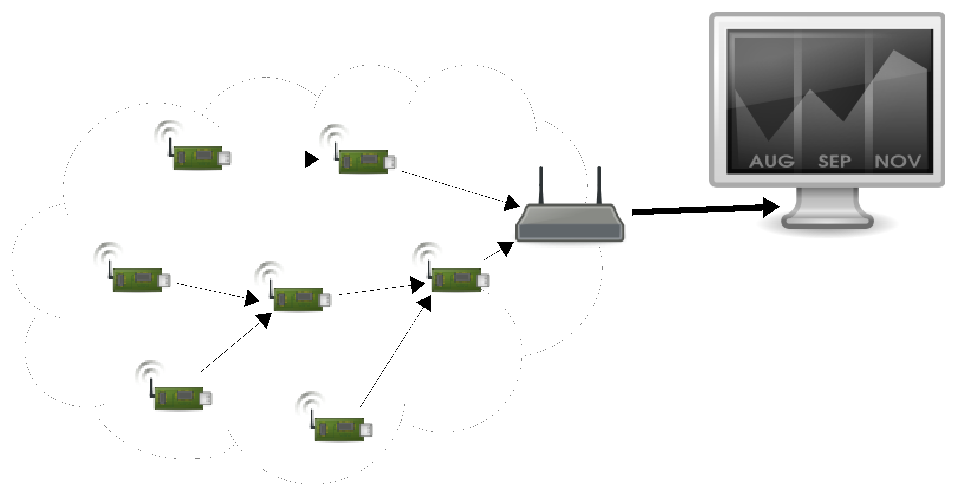
\includegraphics[width=12cm]{wireless_sensor_network}
	\caption{Aufbau eines drahtlosen Sensornetzwerkes}
	\label{fig:wsn}
\end{figure}

Bei drahtlosen Sensornetzen, international auch Wireless Sensor Networks (WSN) genannt, handelt es sich um Netzwerke aus kleinen Sensoren, die ihre Messergebnisse zu einer zentralen Station senden. Die Sensoren helfen dabei einander, die Informationen weiterzureichen (siehe Abbildung \ref{fig:wsn}). So ein drahtloses Sensornetz kann zum Beispiel in einem Gebäude Temperatur- und Luftfeuchtigkeitswerte an eine zentrale Station liefern, die dann die Klimaanlage entsprechend ansteuert. Eine komplette Verkabelung jedes einzelnen Sensors kann dabei je nach Anzahl sehr aufwendig und kostspielig sein. Wenn die Sensoren dazu noch mobil sein sollen, empfiehlt sich eine drahtlose Kommunikation.

Ein Sensor in einem drahtlosen Sensornetz ist ausgestattet mit einer Kommunikationseinheit, die sich selbstständig innerhalb des Netzes konfiguriert und darüber die eingelesenen Messgrößen zu einer zentralen Stelle transportiert.

%%Ein Sensor ist dabei ein typisches Smart Object. Es 
%% Das Steuergerät soll dabei möglichst klein sein, damit es in einem Steckdosengehäuse Platz finden kann. 
%% Der Fernzugriff soll mithilfe des Protokolls IPv6 erfolgen, um zukunftssicher auf die Infrastruktur des Internet verwenden zu können. 

\subsection{Smart Objects}\label{Smart Objects}

Diese Definition von Smart Objects \index{Smart Object} beruht auf \textcite{vasseur10interconnecting}. Dabei handelt es sich um kleine Objekte, die mit folgenden Einheiten ausgestattet sind:

\begin{itemize}
	\itemsep 0pt
	\item eine Form von Sensor und/oder Aktor
	\item ein kleiner Mikrocontroller
	\item eine Kommunikationseinheit
	\item eine Energieversorgung
\end{itemize}

Ein Sensor und/oder Aktor wird benötigt, um mit der Umwelt interagieren zu können. Ein Sensor kann bestimmte Messgrößen erfassen, die dann verarbeitet werden können. Ein Aktor ist das Gegenstück zu einem Sensor. Über ihn kann aktiv die Umwelt beeinflusst werden. Die Kommunikationseinheit befähigt das Smart Object über ein Netzwerk kommunizieren zu können. Es ist dabei möglich mit anderen Smart Objects zu kommunizieren als auch mit weit entfernten Geräten, im Falle des Internets weltweit. Ein kleiner Mikrocontroller übernimmt die Informationsverarbeitung. Dieser nimmt Daten von Sensoren entgegen bzw. steuert den Aktor. Die Kommunikation wird ebenso von ihm geregelt, von einem Sensor gemessene Werte können über das Netzwerk weitergegeben werden. Der Mikrocontroller kann als Kern des Smart Object angesehen werden. Die Energieversorgung ist notwendig, um alle Einheiten ausreichend mit elektrischer Energie zu versorgen.

Alle diese technischen Eigenschaften machen ein Objekt aber noch nicht zu einem Smart Object. Erst die Anwendung und sein Verhalten machen aus einem Objekt mit den obigen Eigenschaften ein Smart Object. Allerdings ist es sehr schwierig, dieses Verhalten zu definieren. Die Anwendungen sind sehr unterschiedlich und es ist völlig unbekannt, wie Smart Objects in der Zukunft eingesetzt werden. Gemeinsam ist allen Anwendungen allerdings, dass Smart Objects mit der physikalischen Umwelt interagieren und über ein Netzwerk kommunizieren. Dieses Verhalten und die obigen technischen Eigenschaften machen ein Smart Object aus.

Von der Kommunikationstechnologie her ähnelt ein Smart Object einem Sensor in einem Sensornetz. Allerdings ist im Gegensatz zu einem Sensornetz ein Netz aus Smart Objects nicht allein auf die Datenübermittlung fokussiert. Bei einem Sensornetz ist der Datenfluss immer vom Sensor ins Netzwerk, wohingegen der Datenfluss bei einem Smart Object bidirektional ist. Der Fokus liegt dabei auf eine Vielzahl von Funktionen insbesondere der Steuerung und Überwachung \citep[Seite 12]{vasseur10interconnecting}. Es ist also die Anwendung, die ein Gerät zu einem Smart Object macht. Aber Entwicklungen, hauptsächlich in der Energieversorgung und Kommunikationstechnik, kommen beiden Forschungsgebieten zugute.


\subsection{Internet-of-Things}

\begin{figure}[htbp]
	\centering
	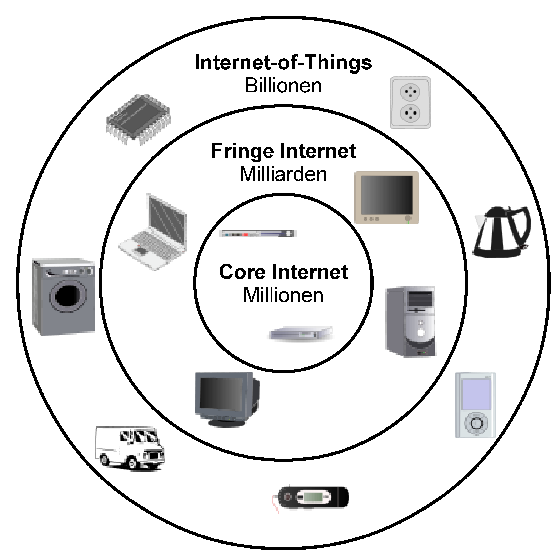
\includegraphics{internet_of_things}
	\caption{Die Internet-of-Things Vision \cite[Figure 1.2]{Bormann:6LoWPAN}}
	\label{fig:internet_of_things}
\end{figure}

Das Internet-of-Things, auch Internet der Dinge genannt, ist eine Vision, wie sich das Internet in Zukunft entwickeln kann. Es soll aus der Vernetzung vieler Kleinstgeräte -- auch oder vielleicht hauptsächlich Smart Objects -- bestehen. \textcite{Bormann:6LoWPAN} betrachten das Internet-of-Things als eine weitere Schale des Internets (Abbildung \ref{fig:internet_of_things}), die gerade anfängt sich heraus zu bilden. Der Kern des Internets (Core Internet) besteht heute aus vielen Routern und Servern, die zusammen Millionen von Teilnehmern ausmachen. Um diesen Kern herum liegt das sogenannte Fringe Internet, was beispielsweise aus privaten Rechnern oder Laptops besteht, aber auch aus lokalen Netzwerken, die zum Internet verbunden werden. Die Teilnehmer des Fringe Internet gehen in die Milliarden. Um dieses Fringe Internet herum beginnt sich eine weitere Schale zu bilden, das sogenannte Internet-of-Things. Auf lange Sicht kann hier mit Billionen von Teilnehmern gerechnet werden. Hauptsächlich bestehen diese Teilnehmer aus IP-fähigen eingebetteten Systemen (embedded systems). Eine so große Zahl an Teilnehmern kann nur mithilfe des Internet Protokolls der Version 6 ans Internet angeschlossen werden, da das bisherige Internet Protokoll der Version 4 keine freien Adressräume mehr zur Verfügung hat.

\section{Theoretische Grundlagen}
\ldots
\section{Kommunikationstechnologien}
\ldots
\section{Betriebssysteme für SmartObjects}
\ldots
\section{Zusammenfassung/Bewertung}
\ldots
%%
%% Beuth Hochschule für Technik --  Abschlussarbeit
%%
%% Kapitel 3 - Konzept / Architektur
%%
%%

\chapter{Konzeption / Architektur} \label{Konzept}


Da die verschiedenen Technologien aufeinander aufbauen, manchmal zueinander kompatibel sind, manchmal inkompatibel sind, werden nachfolgend mögliche Komplettlösungen hergeleitet. Sie werden zuerst kurz vorgestellt, miteinander verglichen und bewertet. Um einen systematischen Entscheidungsprozess zu gewährleisten, werden die möglichen Komplettlösungen mithilfe der Nutzwertanalyse verglichen und bewertet. Der Vorteil der Nutzwertanalyse ist es, dass die Bewertung nachvollziehbar und überprüfbar ist. Nach der Auswertung wird die Lösung ausgesucht, die implementiert werden soll.

\section{Entwurf des eigenen Lösungskonzepts}
\begin{itemize}
\item Darstellung des eigenen Ansatzes, ggf. Abgrenzung von anderen Arbeiten
\item Vor-/Nachteile
\item \ldots
\end{itemize}

\section{Auswahl/Entwurf der Hardware}
\ldots
\section{Auswahl/Entwurf der Software}
\subsection{Entwurf von Lösungsmodulen}
\ldots




%%
%% Beuth Hochschule für Technik --  Abschlussarbeit
%%
%% Kapitel 4 - Implementierung
%%
%%

\chapter{Implementierung} \label{Implementierung}

\section{Aufbau der Implementierung}

Die Implementierung der Lösung erfolgte in zwei Teilen. Es wurde die Hardware erstellt und zeitlich parallel dazu wurde die Software entwickelt. Beide Teile konnten relativ unabhängig voneinander implementiert werden. Die Schnittstelle von Hardware und Software ist das Zigbit-Modul ATZB-24-A2. Auf diesem Modul wird die fertige Software einprogrammiert. Die Hardware versorgt das Modul mit Energie und schaltet nach Softwarevorgaben die Steckdose ein und aus.



\section{Contiki-Verzeichnisstruktur}
%\section{Contiki Verzeichnisstruktur}

Die Contiki-Verzeichnisstruktur besteht aus verschiedenen Unterverzeichnissen, die verschiedene Bedeutungen haben.

\begin{lstlisting}[caption=Contiki-Verzeichnisstruktur mit ausgewählten Unterverzeichnissen]{Contiki Dateistruktur}
/apps                                     
    /ftp                                      
    /ping6                                
    /telnet                               
    /telnetd                              
    /twitter                              
    /webserver                            
    /webserver-nano                       
    ...                                   
/core                                    
    /lib                                  
    /net                                  
    /sys                                  
    ...
/cpu
    /arm
    /avr
    ...
/doc
/examples
    /webserver-ipv6-raven
    ...
/platform
    /avr-raven
    /avr-zigbit
    ...
/tools
\end{lstlisting}

Das Verzeichnis /core beinhaltet das Kernstück von Contiki. Hier wird zum Beispiel das System im Unterverzeichnis /sys definiert. Das beinhaltet das Prozesshandling und Protothreads sowie verschiedene Timer. Ebenfalls befindet sich hier im Unterverzeichnis /net der Netzwerk-Stack aufbauend auf uIP. Zum Netzwerk-Stack gehört auch IEEE 802.15.4 und 6LoWPAN. Im Unterverzeichnis /lib stehen verschiedene libraries zur Verfügung.

In den beiden Verzeichnissen /cpu und /platform ist die unterschiedliche Hardware beschrieben, die von Contiki unterstützt wird. Ein Programm, das auf einem Zigbit-Modul vom Hersteller Atmel geladen werden soll, verwendet die Verzeichnisse /platform/avr-zigbit und /cpu/avr.

Das Verzeichnis /examples beinhaltet Beispielprojekte. Hier gibt es ein Projekt webserver-ipv6-raven. Anhand dieses Beispiels wird deutlich, was notwendig ist, um eine Webserver-Applikation für das Ravenboard zu kompilieren.

Im Hauptverzeichnis gibt es eine Datei Makefile.include. Diese Datei ist Teil des Contiki-Makefile-Systems. Sie wird innerhalb eines Contiki-Projektes aufgerufen und bindet, abhängig von der Konfiguration des Projektes, die richtigen Dateien des Contiki-Systems ein.

\subsection{Übersetzung eines Contiki-Programms}

Ein Programm wird in Contiki mithilfe des Befehls "`make"' übersetzt. Am Beispiel des Projekts webserver-ipv6-raven soll exemplarisch gezeigt werden, wie das Makefile System funktioniert. Durch den Befehl "`make"' wird die Datei Makefile im gleichen Verzeichnis abgearbeitet.

\begin{lstlisting}[caption=Auszug aus examples/webserver-ipv6-raven/Makefile]
ifndef TARGET
  TARGET=avr-raven
  MCU=atmega1284p
endif
all:
  ${MAKE} -f Makefile.webserver TARGET=$(TARGET) NOAVRSIZE=1 webserver6.elf
\end{lstlisting}

Hier wird das TARGET, also die Plattform, und die MCU, die Microcontroller Unit, gesetzt und dann die Datei Makefile.webserver aufgerufen. Dabei wird der Parameter NOAVRSIZE gesetzt, um beim Übersetzen eine zusätzliche Ausgabe zur Speicherbelegung (avr-size) zu unterdrücken. Das Programm wird als Datei webserver6.elf erstellt.

\begin{lstlisting}[caption=Auszug aus examples/webserver-ipv6-raven/Makefile.webserver]
all: webserver6
APPS=raven-webserver raven-lcd-interface
UIP_CONF_IPV6=1
CONTIKI = ../..
include $(CONTIKI)/Makefile.include
\end{lstlisting}

In der Datei Makefile.webserver werden die Applikationen raven-webserver und raven-lcd-interface über die Variable APPS eingebunden. Es wird eine Compiler Variable UIP\_CONF\_IPV6 gesetzt, um IPv6 zu aktivieren, und das Haupt-Makefile Makefile.include wird eingebunden.

\begin{lstlisting}[caption=Auszug aus examples/webserver-ipv6-raven/webserver6.c]
#include "webserver-nogui.h"
/*--------------------------------------------------------------------*/
AUTOSTART_PROCESSES(&webserver_nogui_process);
/*--------------------------------------------------------------------*/
\end{lstlisting}

In der Datei webserver6.c wird ausgewählt, welche Contiki-Prozesse automatisch gestartet werden sollen. In unserem Beispiel ist das der Prozess "`webserver\_nogui\_process"'. Dieser Prozess ist Teil der Applikation raven-webserver.



\subsection{Programmieren eines Mikrocontrollers}


Durch Übersetzung des Contiki-Beispielprojektes webserver-ipv6-raven wird eine Datei "`webserver6.elf"' im ELF Format erzeugt. Hiervon wird eine Kopie "`webserver6-avr-raven.elf"' erstellt. Diese Datei enthält Informationen darüber, was in den Flash und in den EEPROM des AVR Mikrocontrollers geladen werden muss. Ebenfalls beinhaltet es Informationen über das Setzen der Fuse Bits. Fuse Bits sind Einstellungen des Mikrocontrollers, die nicht von der Software geändert werden können. Sie schalten gewisse Funktionen, zum Beispiel woher die Taktfrequenz bezogen wird, ein oder aus.

\begin{lstlisting}[caption=Auszug aus examples/webserver-ipv6-raven/Makefile]
TARGET=avr-raven
MCU=atmega1284p
OUTFILE=webserver6-$(TARGET)
avr-objcopy -O ihex -R .eeprom -R .fuse -R .signature \
            $(OUTFILE).elf $(OUTFILE).hex
avr-size -C --mcu=$(MCU) $(OUTFILE).elf
\end{lstlisting}

Durch zusätzliche Befehle im Makefile wird eine Datei "`webserver6-avr-raven.hex"' erzeugt. Diese Datei enthält den Inhalt, der in den Flash geschrieben werden soll, im Intel-HEX-Format. Mit dem "`avr-size"'-Befehl wird die Anzahl der Bytes angezeigt, die im Flash, im RAM und im EEPROM benötigt werden. Dies kann mit dem zur Verfügung stehenden Speicher verglichen werden.

\begin{lstlisting}[caption=Ausgabe vom Befehl "`avr-size"']
AVR Memory Usage
----------------
Device: atmega1284p

Program:   70874 bytes (54.1% Full)
(.text + .data + .bootloader)

Data:      13013 bytes (79.4% Full)
(.data + .bss + .noinit)

EEPROM:       63 bytes (1.5% Full)
(.eeprom)
\end{lstlisting}

Durch Hinzufügen eines zusätzlichen Befehls ins Makefile kann eine Datei "`webserver6-avr-raven\_eeprom.hex"' erzeugt werden. Diese Datei enthält dann den Inhalt im Intel-HEX-Format, der in den EEPROM geschrieben werden soll. Mit den beiden Dateien im Intel-HEX-Format ist es möglich, den Mikrocontroller mit einem Programmiergerät zu beschreiben, das kein ELF Format lesen kann.

\begin{lstlisting}[caption=Befehl um eeprom.hex zu erzeugen]
avr-objcopy -O ihex -j .eeprom \
            -set-section-flags=.eeprom="alloc,load" --change-section-lma \
            .eeprom=0 $(OUTFILE).elf $(OUTFILE)_eeprom.hex
\end{lstlisting}


Mittels des Programms Atmel Studio 6 werden wahlweise die erzeugten Dateien im Intel-HEX-Format oder die erzeugte Datei im ELF Format in den Flash und in den EEPROM des Mikrocontrollers programmiert. Zu Beginn wurde das Beispielprojekt webserver-ipv6-raven auf den Mikrocontroller AT-Mega1284P eines Atmel Ravenboard programmiert. Dabei wurde die Programmierschnittstelle ISP und das Programmiergerät Atmel STK500 verwendet.

Später bei der entwickelten Hardware wurde die Programmierschnittstelle JTAG und das Programmiergerät Atmel JTAGICE3 verwendet.


% !TEX root = ../Thesis.tex
%%
%%  Hochschule für Technik und Wirtschaft Berlin --  Abschlussarbeit
%%
%% Kapitel 5 - Tests
%%
%%

\chapter{Tests} \label{Tests}

In diesem Kapitel wird die erstellte Lösung getestet und die Entwicklung validiert.
Dazu ist die Testumgebung zu beschreiben. 

Ziel ist der glaubhafte Nachweis der Funktionsfähigkeit, bzw. die quantitative Bewertung
der erstellten Lösung. 

Ein wichtiges Kriterium ist die Nachvollziehbarkeit der Tests. Das heißt, die Tests müssen
so beschrieben sein, dass der Leser der Arbeit die Ergebnisse eigenständig wiederholen und
validieren kann.

\section{Herleitung von Test-Cases}
Herleitung der Testmethodik.

\subsection{Funktionale Tests}
\ldots
\subsection{Leistungstests/Performancetests}
\ldots
\section{Bewertung der Ergebnisse}
\ldots
% !TEX root = ../Thesis.tex
%%
%%  Hochschule für Technik und Wirtschaft Berlin --  Abschlussarbeit
%%
%% Kapitel 6
%%
%%

\chapter{Fazit} \label{Fazit}

In diesem Kapitel wird die erstellte Lösung begutachtet. Es werden Anwendungsmöglichkeiten, allgemein von Smart Objects und speziell für die Implementierung, behandelt. Mögliche Erweiterungen werden vorgeschlagen und ein Fazit der Arbeit wird gezogen.

\section{Analyse der Implementierung}

Die erstellte Lösung wird kritisch begutachtet. Dafür werden zuerst Kostenbetrachtungen bezogen auf die Hardware und auf die Software durchgeführt. Die Ergebnisse fließen in die abschließende Bewertung mit ein. 

\subsection{Kostenbetrachtung}

Um in der Bewertung der Implementierung die Kosten einschätzen zu können, sollen hier zum einem die Hardwarekosten vorgestellt werden. Dazu sollen die einzelnen Materialkosten der verwendeten Bauteile zusammengefasst werden. Um die gesamten Hardwarekosten ermitteln zu können, müssen auch Entwicklungskosten und Fertigungskosten berücksichtigt werden. Fertigungskosten beinhalten dabei die eigentlichen Arbeitsstunden, die für die Fertigung aufgebracht werden müssen, als auch die Investitionskosten für den Fertigungsarbeitsplatz. Weil das sehr abhängig von der Art der Fertigung ist, sei es eine Einzelstückfertigung oder eine Serienfertigung, werden diese Kosten hier nicht näher betrachtet. Die Hardwarekosten werden rein durch die Materialkosten repräsentiert.

Zum anderen sollen die Softwarekosten abgeschätzt werden. Dies wird durch die Ermittlung der Entwicklungskosten für die Contiki-Applikation iec104 erreicht. Anhand eines angenommenen Stundensatzes für einen Softwareentwickler und den aufgewendeten Stunden werden die Kosten für die Entwicklung berechnet.

\subsubsection{Materialkosten}

\begin{table}[htbp]
\small
\caption{Materialkosten Steckdose}
\begin{tabular}{|r|l|l|p{2cm}|p{2cm}|}\hline
  \textbf{\#} & \textbf{Bauteil} & \textbf{Artikelnummer} & \textbf{Einzel-preis in~€} & \textbf{Massen-preis in~€} \\ \hline
  \multicolumn{5}{|l|}{Zigbit-Platine} \\ \hline
  1 & ATZB-24-A2 & 556-ATZB-24-A2 & 25,43 & 14,42 \\ \hline
  1 & Widerstand 100kOhm & 71-CMF60100K00FKEB & 0,206 & 0,099 \\ \hline
  1 & Widerstand 1kOhm & 71-CMF551K0000FHEK  & 0,116 & 0,005 \\ \hline
  1 & Kondensator 3,3uF & 667-EEU-HD1H3R3 & 0,165 & 0,104 \\ \hline
  1 & Spannungsregler LP2950CZ-3.0 & 926-2950CZ-3.0/NOPB & 0,676 & 0,27 \\ \hline
  1 & Steckverbinder FFC 6 Pin & 538-52271-0679 & 1,30 & 0,583 \\ \hline
  2 & Steckverbinder FFC 18 Pin & 538-52271-1879 & 1,71 & 0,94 \\ \hline
  \multicolumn{5}{|l|}{Steckdosen-Platine} \\ \hline
  1 & Kondensator X2 275V & 80-R46KN368050M2M & 0,66 & 0,263 \\ \hline
  1 & Widerstand 560Ohm, 5Watt & 594-AC05W560R0J & 0,38 & 0,198 \\ \hline
  2 & Widerstand 1MOhm & 594-MRS251M1\%TR & 0,074 & 0,038 \\ \hline
  2 & Gleichrichterdiode & 512-1N4004 & 0,076 & 0,025 \\ \hline
  2 & Zener-Diode 24V & 512-1N4749ATR & 0,203 & 0,036 \\ \hline
  1 & Kondensator 470uF & 667-EEU-FR1E471YB & 0,248 & 0,152 \\ \hline
  1 & NPN-Transistor BC547B & 512-BC547B & 0,186 & 0,05 \\ \hline
  1 & Widerstand 220kOhm & 271-220K-RC & 0,125 & 0,012 \\ \hline
  \multicolumn{5}{|l|}{Steckdosen-Gehäuse} \\ \hline
  1 & Tchibo Digitale Zeitschaltuhr & 4 043002 669758 & 5,99 & 5,99 \\ \hline
  \multicolumn{5}{|l|}{} \\ \hline
  \multicolumn{3}{|l|}{\textbf{Gesamtpreis}} & \textbf{38,61} & \textbf{24,27} \\ \hline
\end{tabular}
\label{tab:hardwarekosten}
\end{table}

In Tabelle \ref{tab:hardwarekosten} sind die Bauteile aufgelistet, die zum Erstellen der Steckdose verwendet wurden. Sie benennt das Bauteil und zeigt die Anzahl an, die verbaut wurden. Die Bauteile wurden -- bis auf die Tchibo Steckdose -- vom Handelsunternehmen Mouser Electronics bezogen. In der dritten Spalte ist die entsprechende Artikelnummer aufgelistet. Die vierte Spalte zeigt den Preis bei dem Bezug von nur einem Bauteil. Bei einer Massenfertigung der Steckdose werden andere Preise angeboten. Der Stückpreis bei einer Bestellung von 1000 Fertigungssätzen ist in der letzten Spalte aufgelistet. Die Preise wurden am 06.05.2013 abgefragt und sind inklusive Mehrwertsteuer.

Die Gesamtmaterialkosten der verwendeten Bauteile betragen 38,61€. Nicht berücksichtigt sind Verbrauchsmaterialien. Dazu zählen die Leiterplatte für die Zigbit-Platine, die aus einer vorhandenen Lochrasterplatine ausgesägt wurde, Leitungen für die Verkabelung und Lötzinn. Diese Kosten sollen hier vernachlässigt werden. Bei einer Kalkulation für eine Fertigung in einem Unternehmen müssen diese als Materialgemeinkostenzuschlag zu den Materialkosten hinzugefügt werden. Zusammen mit den Fertigungskosten, also die Arbeitskosten, die zum Fertigen der Steckdose notwendig sind, und den Verwaltungs- und Vertriebsgemeinkostenzuschlag ergeben sich die Selbstkosten je Stück.

\subsubsection{Entwicklungskosten iec104}

Um den Aufwand von einer Contiki-Applikation abzuschätzen, sollen beispielhaft die Entwicklungskosten der implementierten Applikation iec104 ermittelt werden. Zum Ermitteln der Kosten, muss der Stundensatz des Entwicklers mit der Zeit in Stunden multipliziert werden, die dafür notwendig ist, eine solche Applikation zu programmieren. Dazu gehört eine Designphase, die eigentliche Programmierung und eventuelle Fehlerkorrekturen. Weil die Kosten proportional zur Zeit sind, soll nur diese betrachtet werden. Es wird geschätzt, dass für die Entwicklung der Applikation iec104 etwa drei bis vier Mannwochen benötigt wurden. Die Schätzung wird dadurch erschwert, dass nicht kontinuierlich an der Entwicklung gearbeitet wurde. Die Arbeit daran wurde öfter durch andere notwendige Arbeiten unterbrochen.

Deswegen soll noch eine quantitative Bewertung anhand der Anzahl geschriebener Zeilen Quellcode LOC (Lines Of Code) stattfinden. In der Praxis ist solch eine Bewertung, also der Rückschluss von den LOC auf den Aufwand, allerdings problematisch. Die Zeit, die für die Designphase verwendet wird, wird nicht berücksichtigt. Eine überlegte und optimierte Programmierung benötigt tendenziell weniger LOC. Die Qualität der Programmierung wird auch nicht bewertet. Verschiedene Programmiersprachen und individuelle Programmierstile wirken sich ebenso auf die LOC aus. 

Trotzdem gibt es Faustformeln, die einen Zusammenhang zwischen der Anzahl geschriebener Zeilen Quellcode LOC und der eingesetzten Entwicklungszeit sehen. Nach \cite[Seite 305]{Ludewig:SoftwareEngineering} wird in einem Softwareprojekt nach n Stunden Aufwand -- wobei hier der Gesamtaufwand gemeint ist, nicht die reine Programmierungszeit -- ein System mit zwei mal n LOC erzeugt. Ein studentisches Projekt, das nicht kommerziell vertrieben werden soll, kann in der gleichen Zeit in etwa die dreifache Anzahl an LOC liefern. Dort können demnach mit jeder Stunde Aufwand in etwa sechs LOC entwickelt werden.

Um nach dieser Faustformel herauszufinden, wie viele Stunden in die Entwicklung der Contiki-Applikiation iec104 eingeflossen sind, werden die Anzahl an Zeilen Quellcode ermittelt. Die Contiki-Applikation iec104 besteht aus 14 Dateien:
\begin{itemize}
	\itemsep 0pt
	\item 1 Makefile
	\item 7 Header-Dateien
	\item 6 C-Dateien
\end{itemize}

Insgesamt enthalten diese Dateien 1011 Zeilen. Wenn die 211 Leerzeilen und 112 Kommentarzeilen abgezogen werden, bleiben 688 Zeilen Quellcode. Nach der Faustformel oben ergibt sich eine Entwicklungszeit von etwa 115 Stunden. Bei der Annahme von einem Stundensatz von 100€ ergeben sich Entwicklungskosten von 11.500€. Bei einer Wochenarbeitszeit von 40 Stunden, ergeben sich ungefähr 3 Mannwochen, die notwendig sind, um die Contiki-Applikation iec104 zu entwickeln. Das deckt sich in etwa mit den Erfahrungen aus dieser Arbeit.



\section{Anwendungsmöglichkeiten}

Dieses Kapitel stellt zuerst allgemein verschiedene Anwendungsbereiche von Smart Objects vor. Darauffolgend wird erörtert, in welchen Anwendungsbereichen die erstellte Lösung eingesetzt werden könnte. Anhand der Erfahrung, die bei der Implementierung gemacht wurden, werden mögliche Erweiterungen behandelt.

\subsection{Anwendungsbereiche von Smart Objects}

Smart Objects können in einer Vielzahl von Anwendungsbereichen eingesetzt werden, da sie sehr flexibel in ihrer Beschaffenheit sind. Die Programmierung kann individuell angepasst werden. Durch die Verwendung der richtigen Sensoren und Aktoren sind sie für verschiedenste Einsatzbereiche verwendbar. Nachfolgend sollen folgende fünf mögliche Anwendungsbereiche kurz beschrieben werden:

\begin{itemize}
	\itemsep 0pt
	\item eHome-Bereich
	\item Gebäudeautomation
	\item Industrieautomatisierung
	\item Logistik
	\item Smart Grid
\end{itemize}

Der eHome-Bereich ist ein Bereich in dem sich mehrere proprietäre Lösungen verbreitet haben, die oft nicht untereinander kompatibel sind. Dies kann auch ein Mitgrund dafür sein, dass sich die Heimautomatisierung bisher nicht so entwickelt hat wie vor etwa 7-9 Jahren prognostiziert \citep[360]{vasseur10interconnecting}. Wichtig ist auch, gerade im eHome-Bereich, eine einfache Installation der Geräte. Nur wenn ein Endnutzer ohne spezielles Expertenwissen Geräte in Betrieb nehmen und verwenden kann, wird sich eine Lösung durchsetzen können. Mögliche Einsatzgebiete von Smart Objects im eHome-Bereich sind zum Beispiel Steuerungen von Licht, der Heizung, von Fenster, von Rollläden und von Türschlössern.

Der eHome-Bereich wird für private Wohnhäuser eingesetzt. Im Gegensatz dazu zielt die Gebäudeautomation eher auf den professionellen Einsatz in großen Gebäuden meist im Zusammenspiel mit einem visualisierten Gebäudemanagementsystem. \textcite[Seite 304ff]{Vermesan:TheInternetOfThings} beschreiben unter dem Titel "`Smart IPv6 Building"' verschiedene Forschungsprojekte, die die Verwendung von IPv6 in der Gebäudeautomation untersuchen. Unter anderem wird auch das Hobnet-Projekt erwähnt, das spezielle Anwendungsfälle von Smart Objects in der Gebäudeautomation untersucht. Hier kommt auch 6LoWPAN zum Einsatz. Allgemein sind die Ziele einer Gebäudeautomation Energieeinsparungen, Sicherheit und Komfortgewinn.


Der Bereich Smart Grid wird einer der größten Anwendungsbereiche für Smart Objects werden \citep[Seite 271ff]{Hersent:TheInternetOfThings}. Seit mehreren Jahren geht der Trend in der Stromerzeugung immer mehr in Richtung erneuerbaren Energiequellen wie Windkraftanlagen oder Photovoltaikanlagen. Diese sind aber im Gegensatz zu klassischen fossilen Kraftwerken dezentral aufgestellt. Das führt zu einem erheblichen Umbruch in der Stromnetzführung. Die Energie wird nicht allein an wenigen zentralen Örtlichkeiten durch große Kraftwerke, sondern auch dezentral durch kleine teils privat teils kommerziell geführten Energiequellen erzeugt. Das erschwert die Kraftwerksregelung und die Leitung des Lastflusses. Um trotzdem eine gute Netzstabilität zu gewährleisten, muss das Stromnetz intelligenter und vielfältiger überwacht und gesteuert werden.

Eine Maßnahme dabei ist das Smart Metering. Stromverbrauchszähler liefern über eine Kommunikationsschnittstelle den aktuellen Energieverbrauch an das Energieversorgungsunternehmen. Solche Art intelligente Zähler existieren schon länger für große Energieverbraucher wie Produktionsbetriebe, seit einigen Jahren werden Smart Meter auch für Privathaushalte angeboten.


\subsection{Anwendungsmöglichkeiten für die Implementierung}


Das Protokoll IEC104 ist ein Fernwirkprotokoll aus dem Bereich der Energieautomatisierung. Der Bereich Smart Grid ist also ein klassischer Anwendungsfall für dieses Protokoll. An ein zentrales Leitsystem werden Informationen übertragen und Steuerbefehle entgegen genommen. Allerdings wird der Zugriff auf eine Steuerung von einem elektrischen Verbraucher im Privathaushalt für ein Energieversorgungsunternehmen nicht von Bedeutung sein. Ein möglicher Anwendungsfall liegt eher in einem Smart Meter. Hier könnten mittels IEC104 Verbrauchsstände übertragen werden. Zusätzlich wäre in Absprache mit dem Privathaushalt eine Steuerung möglich. Genaue Anwendungsfälle müssen noch erprobt werden. Denkbar wäre eine Notabschaltung einer lokalen Photovoltaikanlage, wenn mehr Energie ins Stromnetz eingespeist wird als dort verbraucht wird bzw. in andere Stromnetzregionen abgeführt werden kann. Ebenfalls denkbar ist eine gezielte Steuerung von größeren Energieverbrauchern, bei denen der Einsatz zeitlich flexibel ist (Demand Side Management). Beispiele dafür sind die Waschmaschine oder die Batterie eines Elektrofahrzeugs. Bei einer großer Netzauslastung können diese steuerbaren Verbraucher zurückgefahren werden. Das Energieversorgungsunternehmen muss dann weniger Reserven für Spitzenlast vorhalten. So hilft eine intelligente Netzführung dabei, Kosten in der Energieerzeugung zu reduzieren.

\subsection{Erweiterungsvorschläge für die Implementierung}

Die erstellte Lösung ist ein Prototyp, der beispielhaft implementiert worden ist. Während der Arbeit sind mehrere Ideen entstanden, wie die Implementierung verbessert oder erweitert werden kann. Zuerst werden Vorschläge für die IEC104-Slave-Applikation aufgelistet.

\begin{itemize}
	\itemsep 0pt
	\item Informationsmeldungen mit Zeitstempel
	\\Die Statusänderung der Steckdose erfolgt aktuell über den Datentyp M\_SP\_NA\_1 (Type Ident 1): Einzelbitmeldung ohne Zeitstempel. Eine Verbesserung wäre die Verwendung des Datentyps M\_SP\_TB\_1 (Type Ident 30): Einzelbitmeldung mit dem Zeitstempel CP56Time2a. Hier wird zusätzlich ein Zeitstempel mit Jahr, Monat, Tag, Stunde, Minute, Sekunde und Millisekunde übertragen. So ist der exakte Zeitpunkt der Statusänderung bekannt. Voraussetzung dafür ist aber, dass die Steuerung mit der aktuellen Zeit synchronisiert ist. Über IEC104 existiert dafür eine Möglichkeit mit dem Datentyp C\_CS\_NA\_1 (Type Ident 103): Zeitsynchronisationsbefehl. Ein Zeitstempel wird vom IEC104-Master zum IEC104-Slave gesendet und dort übernommen. Weil die Übertragungszeit dabei aber nicht berücksichtigt wird, ist die Verwendung vom IEC-Standard nur bedingt empfohlen. In der Praxis wird oft das Protokoll NTP (Network Time Protocol) verwendet. Eine Implementierung von NTP im Betriebssystem Contiki existiert bereits \cite{Contiki-syslog}.
	\item interne Statusinformationen des Contiki Betriebssystems
	\\Das Modul iec104-para kann mit zusätzlichen Informationsobjekten erweitert werden. Zusätzliche interne Statusinformationen wie die Anzahl der laufenden Prozesse, TCP/IP-Verbindungen oder die Betriebszeit könnten übertragen werden. Für Messwerte gibt es bereits den Datentyp M\_ME\_NA\_1 (Type Ident 9): Messwert, normalisiert und ohne Zeitstempel. Weitere Datentypen können implementiert werden.
\end{itemize}

Eine weitere Verbesserungsmöglichkeit betrifft nicht die Implementierung selbst sondern dem Testaufbau. Als 6LoWPAN-Router wurde ein handelsüblicher PC mit einer Linux-Installation verwendet. Als 6LoWPAN-Schnittstelle wurde ein USB-Stick RZUSBSTICK von Atmel verwendet, der auf dem PC eine Ethernet-Schnittstelle simuliert. Unter anderem hat das den Nachteil, dass auf dem PC der 6LoWPAN-Netzwerkverkehr nicht beobachtet werden kann, weil nur der simulierte Ethernet-Verkehr sichtbar ist. Es wird aber aktuell daran gearbeitet, 6LoWPAN direkt im Linux-Kernel zu implementieren \citep{Ott2012}. Eine eingeschränkte Variante wird schon seit der Kernel Version 3.2.46 unterstützt und laufend erweitert. Als Funkchips werden der MRF24J40 von Microchip und der AT86RF230 von Atmel, der auch im Zigbit-Modul verbaut ist, unterstützt. \citeauthor{Ott2012} stellt eine Hardware vor bestehend aus einem BeagleBone und einem MRF24J40MA Funkchip. Damit kann 6LoWPAN nativ unter Linux verwendet werden ohne zusätzliche Hardware und ohne ein zusätzliches Betriebssystem. Es ist allerdings nicht bekannt, ob es Interoperabilitätsprobleme zwischen der 6LoWPAN-Implementierung im Linux-Kernel und im Contiki-Betriebssystem gibt.

\section{Fazit}

Es konnte gezeigt werden, dass eine internetfähige Steuerung mithilfe eines 8-bit Mikrocontrollers implementiert werden kann. Das Betriebssystem Contiki stellt dazu den notwendigen TCP/IP-Stack und andere Werkzeuge und Hilfsmittel zur Verfügung. Eine Webserver-Anwendung und eine Vielzahl anderer Anwendungen sind Teil des Betriebssystems. Mit der Contiki-Appliktation iec104 wurde gezeigt, dass die Implementierung des Protokolls IEC104 in einer limitierten Umgebung durchaus möglich ist. Auch die Verwendung von IEC104 im Zusammenspiel mit IPv6 hat funktioniert. Bisher war keine Implementierung von IEC104 über IPv6 bekannt. Generell zeigt die Contiki-Applikation iec104, dass die Implementierung neuer internetfähiger Anwendungen möglich und nicht aufwendiger als bei anderen Betriebssystemen ist. Die geringen Ressourcen müssen allerdings bei der Programmierung berücksichtigt werden.

Bei der Implementierung ist der 8KByte große RAM-Speicher die markanteste Ressourcengrenze. Die Auslastung beträgt 88,9\%. Das Hinzufügen von zusätzlichen Contiki-Applikationen oder das Erweitern der Applikation iec104 ist deswegen nicht ohne Weiteres möglich. Durch den Einsatz von anderer Hardware mit einem größeren RAM-Speicher kann dieses Problem umgangen werden. So steht bei dem AVR Ravenboard mit 16KByte doppelt so viel RAM-Speicher zur Verfügung. Der Hersteller Redwire bietet mit dem Econotag ein fertiges Modul mit USB-Schnittstelle an. Verwendet wird der Freescale MC13224V, der einen 32-bit ARM7 Mikrocontroller mit einer IEEE-802.15.4-Schnittstelle kombiniert. Er verfügt über 128KByte Flash- und 96KByte RAM-Speicher. Das Betriebssystem Contiki unterstützt diese Modul über die Platform redbee-econotag. Beide, das AVR Ravenboard und das Econotag, sind aber für den Einbau in die verwendete Steckdose zu groß.

%\cite{ko11beyond}: In this paper we present two interoperable implementations of the IPv6 protocol stack for LLNs for two leading sensor network operating systems: Contiki and TinyOS. We demonstrate that the two implementations interoperate, but also show that interoperability is not enough. Rather, we expose the fact that subtle differences in different layers of the protocol stack can affect the resulting system performance. 

Als Kommunikationstechnologie wurde 6LoWPAN verwendet. Es scheint ideal für den Einsatz bei ressourcenbeschränkten Geräten zu sein. Anfang dieses Jahres hat die ZigBee Alliance die Spezifikation ZigBee IP veröffentlicht \citep{zigbee-ip}. Damit werden unter der Verwendung von 6LoWPAN vermaschte drahtlose IPv6-Netzwerke unterstützt. Dies ist ein Beispiel dafür, dass die Verwendung von 6LoWPAN in vielen Bereichen voranschreitet. Eine weitere Entwicklung, die die Verbreitung von 6LoWPAN unterstützt, ist die Spezifizierung des Protokolls RPL \citep{RFC6550}. RPL ist ein Routing-Protokoll, das für verlustbehaftete Sensornetze entwickelt worden ist. Die speziellen Anforderungen konnten von existierenden Routing-Protokolle wie OSPF oder RIP nicht erfüllt werden. Die Implementierung von RPL im Betriebssystem Contiki wird ContikiRPL genannt \citep{tsiftes10rpl}.

Sehr wichtig für die weitere Verbreitung von 6LoWPAN ist die Interoperabilität von verschiedenen Implementierungen. \textcite{ko11beyond} haben zwei unabhängige Implementierungen, Contiki und TinyOS, zusammen getestet. Die Interoperabilität zwischen beiden war gegeben, allerdings hatten kleine Unterschiede im jeweiligen Protokollstack einen Einfluss auf die Gesamtsystemleistung. Neben der Interoperabilität ist die Leistungsfähigkeit bei dem Zusammenspiel verschiedener Implementierungen von Bedeutung.

Als weitere Schwierigkeit kommt hinzu, dass viele Implementierungen den Funkempfänger so oft wie möglich ausschalten. Im Betriebssystem Contiki steht diese Funktionalität unter dem Namen ContikiMAC zur Verfügung. So kann der Energieverbrauch um bis zu 80\% reduziert werden \citep{dunkels11contikimac}. Das gesteuerte Ausschalten des Funkempfängers hat allerdings einen markanten Einfluss auf das Kommunikationsverhalten im Netzwerk. Weil keine Spezifikationen oder Standards für diese Funktionalität existieren, verhalten sich Implementierungen sehr verschieden. \textcite{dunkels11adhoc} beschreiben, dass das Zusammenspiel von Kommunikationstechnologie und Ausschaltverhalten des Funkempfängers ein wichtiges Forschungsgebiet für das Internet-of-Things ist.

%Vergleich mit Geschichte des Elektromotors:
%http://www.udo-leuschner.de/rezensionen/rf9809dittmann.htm
%Entwicklung des elektrischen Netzes -> elektrische Energie war überall im Haushalt verfügbar. Dadurch konnte der Elektromotor quasi die alleinige Rolle des mechanischen Energielieferanten im Haushalt übernehmen. Am Anfang wurden große Elektromotoren verkauft, an die verschiedene Geräte angeschlossen werden konnten. Mittlerweile hat jedes Gerät einen kleinen Elektromotor. Das Bewusstsein seiner Existenz ist für den Verbraucher dadurch aber noch gesunken, die Technik verschwindet im Hintergrund. Schon seit Anfang der Siebziger Jahre besaß jeder Haushalt 15 bis 20 Elektromotoren.
%-> Die Technik muss in den Hintergrund treten. Darf quasi nicht bemerkt werden. Dann kann sie erfolgreich sein und sich durchsetzen.

%vermutlich wird es immer eine große Mischung aus Technologien geben.

%sonstige Vorschläge zur weiteren Forschung


%% Anhang
\cleardoubleoddpage
\appendix
% !TEX root = ../Thesis.tex
%%
%%  Hochschule für Technik und Wirtschaft Berlin --  Abschlussarbeit
%%
%% Anhang
%%
%%%%%%%%%%%%%%%%%%%%%%%%%%%%%%%%%%%%%%%%%%%%%%%%%%%%%%%%%%%%%%%%%%%%%


\chapter{Der Blindtext}


Weit hinten, hinter den Wortbergen, fern der Laender Vokalien und Konsonantien leben die Blindtexte. Abgeschieden wohnen Sie in Buchstabhausen an der Kueste des Semantik, eines grossen Sprachozeans. Ein kleines Baechlein namens Duden fliesst durch ihren Ort und versorgt sie mit den noetigen Regelialien. Es ist ein paradiesmatisches Land, in dem einem gebratene Satzteile in den Mund fliegen. Nicht einmal von der allmaechtigen Interpunktion werden die Blindtexte beherrscht - ein geradezu unorthographisches Leben.

Eines Tages aber beschloss eine kleine Zeile Blindtext, ihr Name war Lorem Ipsum, hinaus zu gehen in die weite Grammatik. Der grosse Oxmox riet ihr davon ab, da es dort wimmele von boesen Kommata, wilden Fragezeichen und hinterhaeltigen Semikoli, doch das Blindtextchen liess sich nicht beirren. Es packte seine sieben Versalien, schob sich sein Initial in den Guertel und machte sich auf den Weg. Als es die ersten Huegel des Kursivgebirges erklommen hatte, warf es einen letzten Blick zurueck auf die Skyline seiner Heimatstadt Buchstabhausen, die Headline von Alphabetdorf und die Subline seiner eigenen Strasse, der Zeilengasse. Wehmuetig lief ihm eine rethorische Frage ueber die Wange, dann setzte es seinen Weg fort.
Unterwegs traf es eine Copy. Die Copy warnte das Blindtextchen, da, wo sie herkaeme waere sie zigmal umgeschrieben worden und alles, was von ihrem Ursprung noch uebrig waere, sei das Wort und und das Blindtextchen solle umkehren und wieder in sein eigenes, sicheres Land zurueckkehren. Doch alles Gutzureden konnte es nicht ueberzeugen und so dauerte es nicht lange, bis ihm ein paar heimtueckische Werbetexter auflauerten, es mit Longe und Parole betrunken machten und es dann in ihre Agentur schleppten, wo sie es fuer ihre Projekte wieder und wieder missbrauchten. Und wenn es nicht umgeschrieben wurde, dann benutzen Sie es immernoch.
%%%%%%%%%%%%%%%%%%%%%%%%%%%%%%%%%%%%%%%%%%%%%
%%%%%%%%%%%%%%%%%%%%%%%%%%%%%%%%%%%%%%%%%%%%%
%%%%%%%%%%%%%%%%%%%%%%%%%%%%%%%%%%%%%%%%%%%%%


%% Abkürzungsverzeichnis
% 	Befehl: makeindex Thesis.nlo -s nomencl.ist -o Thesis.nls
%
% !TEX root = ../Thesis.tex
%%
%%  Hochschule für Technik und Wirtschaft Berlin --  Abschlussarbeit
%%
%%  Abkürzungsverzeichnis
%%
%% Vorgeplänkel nach
%% http://blog.stefan-macke.com/2006/05/03/abkurzungsverzeichnis-mit-latex/
%%%%%%%%%%%%%%%%%%%%%%%%%%%%%%%%%%%%%%%%%%


\acro{EU}{Europäische Union}
\acro{6LoWPAN}{IPv6 over Low power Wireless Personal Area Network}
\acro{AC}{Alternating Current (Wechselstrom)}
\acro{ANSI}{American National Standards Institute}
\acro{PDU}{Protocol Data Unit}
\acro{API}{Application Programming Interface}
\acro{APS}{Application Support Sublayer (ZigBee)}
\acro{ASDU}{Application Service Data Unit}
\acro{BAN}{Body Area Network}
\acro{BSD}{Berkeley Software Distribution}


\cleardoublepage
\markboth{\nomname}{\nomname}
\printnomenclature

%% Abbildungsverzeichnis
\listoffigures \clearpage

%% Tabellenverzeichnis
\listoftables \clearpage

%% Quelltextverzeichnis
\lstlistoflistings \clearpage

%% Stichwortverzeichnis
%	Befehl: makeindex Thesis
%
\printindex \clearpage

%% Literaturverzeichnis
%	Befehl: biber Thesis
%
\printbibliography[heading=bibintoc, title={\babel{Literaturverzeichnis}{Bibliography}}]
\clearpage
%Literaturverzeichnisse getrennt nach Stichwort
%\printbibliography[heading=bibintoc, keyword={book}, title={Literaturverzeichnis}]\clearpage
%\printbibliography[heading=bibintoc, keyword={online}, title={Onlinequellen}]\clearpage
%\printbibliography[heading=bibintoc, keyword={image}, title={Bildquellen}]\clearpage

%% Erklärung zur Eigenständigkeit
% !TEX root = Thesis.tex
%%
%%  Hochschule für Technik und Wirtschaft Berlin --  Abschlussarbeit
%%
%%  Erklärung zur Eigenständigkeit
%%
%%%%%%%%%%%%%%%%%%%%%%%%%%%%%%%%%%%%%%%%%%%%%%%%%%%%

\addchap{Eigenständigkeitserklärung}

Hiermit versichere ich, dass ich die vorliegende \thethesistyp{} selbstständig und nur unter
Verwendung der angegebenen Quellen und Hilfsmittel verfasst habe. 
Die Arbeit wurde bisher in gleicher oder ähnlicher Form keiner anderen Prüfungsbehörde vorgelegt.

\vskip 1cm

Berlin, den \thedatum

\vskip 1.5cm

\theautor

\end{document}